\documentclass[conference]{IEEEtran}
\usepackage{amssymb}
\usepackage{amsmath}
\usepackage{graphicx}
\usepackage{wasysym}
\usepackage{siunitx}
\usepackage{tabularx, booktabs}
\usepackage[draft]{hyperref}
\hyphenation{op-tical net-works semi-conduc-tor}

\DeclareMathOperator*{\argmax}{\arg\!\max}
\DeclareMathOperator*{\softmax}{\texttt{softmax}}

\begin{document}

\renewcommand{\figureautorefname}{Fig.}
\newcommand{\subfigureautorefname}{Fig.}
\renewcommand{\sectionautorefname}{Section}
\renewcommand{\subsectionautorefname}{Section}


\title{EEL6935 Course Project Final Report \\
    Sentiment Analysis}
\author{\IEEEauthorblockN{
    Caleb Bryant\IEEEauthorrefmark{1},
    Jixin Feng\IEEEauthorrefmark{2}}
\IEEEauthorblockA{Department of \\
    \IEEEauthorrefmark{1} Computer \& Information Science \& Engineering\\
    \IEEEauthorrefmark{2} Electrical \& Computer Engineering\\
    University of Florida,
    Gainesville, FL, 32611\\
    Email: \texttt{{\small\{cal2u,fengjixin\}}@ufl.edu}}}

\maketitle

\begin{abstract}
    The volume of text on the Internet -- unstructured text especially --
    is increasing with drastic speed everyday. Unlike human brains, traditional 
    computer programs have a much more limited ability to extract useful
    information from unstructured text with satisfactory precision.
    While traditional machine learning methods have had some success
    tackling NLP problems with ``bag of words'' models and feature engineering,
    deep learning and the subsequent development of robust word embeddings have shown
    promising results and have made substantial ground towards replacing older methods.
    In this course project for EEL6935 Big Data Ecosystems, we implemented a sentence 
    classification program for sentiment analysis based on Long-Short Term Memory Network 
    (LSTM) and compare the performance with a logistic regression based baseline model. 
    In addition, we also created a web application able to do real-time sentiment analysis
    based on the model we created. 
    
\end{abstract}

\IEEEpeerreviewmaketitle

\section{Introduction}
\label{intro}
    With the tremendous volume of unstructured text generated everyday, both on and off
    the internet, the amount of attention devoted to processing and extracting useful information
    from it has been constantly increasing. It is predicted that by 2020 the
    total data volume of the ``digital universe'' will increase to 40 ZB
    ($40\times 10^{21}$ bytes), which is about 50 times larger than that is was in
    year 2010\cite{gantz2012digital}. Most of the text will be generated by
    sources like the news media, social networks, medical facilities, etc.

    Although this text data is a valuable source of information
    and can be easily comprehended by humans, current computational methods
    continue to struggle extracting information from unstructured text 
    sources.
    Hence effective methods to process and analyze unstructured text data are
    desperately needed.

    In this course project, we are targeting a specific domain of text analysis
    problems -- sentiment analysis. The goal of sentiment analysis is to assign
    proper pre-defined sentiment labels to a given text, so that the emotion behind the
    sentence can be represented and then categorized\cite{allahyari2017brief}.
    Mathematically, the classification model can be represented as:
    $$f:\mathcal{D}\rightarrow\mathcal{L}$$
    w $\mathcal{D}=\{d_0, d_1,\ldots, d_{n-1}\}$ is the set of sentences
    , and $\mathcal{L}=\{l_0, l_1,\ldots, l_{k-1}\}$ is the set of labels.
    Depending on whether multiple labels are allowed to be assigned to a document, the
    classification is called soft or hard\cite{gopal2010multilabel}. When conducting sentiment 
    analysis, the set of labels is usually binary, and they can be used
    to model the overall opinion the subject received. Movie reviews, for example,
    can be labeled as positive or negative\cite{pang2002thumbs}.

    In cases w t is an uneven class distribution, the performance
    of a sentiment analysis system can be evaluated with its
    F-1 score, which can be defined as\cite{forman2003extensive}:
    $$F_1=\frac{2}{\frac{1}{r}+\frac{1}{p}}=\frac{2pr}{p+r}$$
    w $p=\frac{tpr}{tpr+fpr}$ stands for precision and $r=\frac{tpr}{tpr+fnr}$
    stands for recall.

    Historically, sentiment analysis has been done via statistical
    and machine learning methods like Naive Bayes, k-nearest neighbors, decision
    trees, SVM, and so on. In this report, we decide to compare the performance of
    sentence classifier based on different techniques: 
    classic Bag-of-Words\cite{pang2002thumbs},
    Convolutional Neural Network (CNN)\cite{kim2014convolutional} 
    and Long Short-Term Memory (LSTM)\cite{barnes2017assessing}.
    
    We divided our project into two stages: the back-end of sentiment analysis
    and a web-based front-end. The backend program is designed to implement 
    LSTM and compare its performance with the Logistic Regression as a baseline
    of performance. The front-end web application is build with Flask, a 
    a micro web development framework for Python.
    
    The dataset we used to train the system is Stanford Large Movie Review 
    Dataset\cite{maas2011learning}. It's a data set with 25,000 highly polarized
    movie reviews for training purpose and another 25,000 reviews for testing.
    Both raw text and bag-of-words formats of data are included in this dataset
    
    The report is organized as follows: 
    A brief introduction of related research contribution is in \autoref{related}.
    system architecture and different analysis approaches are introduced and compared 
    in \autoref{model}.
    The benchmarks used for evaluating the performance are explained in 
    \autoref{performance}.
    Our simulation environment, dataset, simulation result are presented in 
    \autoref{simulation}. The source code of our program, report and 
    presentation in \LaTeX, as well as the web-application are introduced in \autoref{web}.
    The team coordination and the conclusion of this paper is in \autoref{conclusion}.
    
\section{Related Work}
\label{related}
\subsection{Early Research}
    Sentiment analysis has been actively studied for a long time. At the very beginning
    of its research, classifying sentiment of a document is still a very challenging
    task, so earlier research are mostly focus on classifying document based on their 
    publisher, style, etc.\cite{biber1991variation}. Later in the 90s, researchers 
    were able to classify the genre 
    of text\cite{karlgren1994recognizing,kessler1997automatic}, 
    which is one step closer to the sentiment of the text
    than merely publisher and style of the text. Detecting whether
    the text includes a subjective opinion was not generally possible until early 
    2000s\cite{hatzivassiloglou2000effects}. This marks the beginning of 
    sentiment analysis. Most of the early attempts try to  classify by detecting 
    the sentiment of the entire piece of text\cite{pang2002thumbs,pang2005seeing}. 
    This is relatively easy to achieve but may lost track of the detailed sentiment
    or mixed sentiment\cite{lu2011multi}.
    With the help of significantly improved
    computation power of CPU and GPUs, neural network related techniques 
    started to show great potential in the sentiment analysis 
    domain\cite{kim2014convolutional,barnes2017assessing}.

\subsection{Application in Business Domain}
    Sentiment analysis on reviews has huge application potential. In the domain of 
    shopping for example, more and more consumers nowadays are making 
    purchase decisions about a product not only based on the self introduction of the 
    product but the reputation summarized by the review of it. And the research
    shows that online review of a product can even affect the off-line shopping
    behavior\cite{lipsman2007online}. According to a survey of more than 2000 
    American adults, more than 80\% of internet users (about 60\% of American) 
    does online research before making an off-line purchase at least once per year.
    And among all the online reviews read by internet users, about 73\% to 87\% reviews
    have significant influence on purchasing behaviors especially in the domain
    of restaurant and hotel\cite{pang2008opinion}.
    
    Because online reviews possess such great potential of influence of purchasing
    behavior. The vendors are showing increasing amount of interests of studying them
    too. A white paper published back in 2006\cite{kim2006forrester} shows that 
    there were estimated 75,000 blogs and 1.2 million online posts generated 
    everyday, and that was more than 10 years ago. A blog post published by twitter
    in 2013 shows that the average TPS (tweets per second) was 5,700 and the record
    of 143,199 TPS was created on Aug. 16 2013\cite{tps2013}. With such big number of
    new text generated everyday, any small disturbance of public opinion on any subject
    may bring significant impact on people's behavior.
    
    With the evolvement of online media streaming service, reviews generated from
    from watching movie and online media has become one of the major component of 
    online review. A press release by YouTube claims that with more than 1 billion
    users from 88 countries and speaking 76 languages, there are 1 billion
    hours of YouTube Video has been watched daily. These users' rate and review of 
    video content can be a good source for business decision making. 
    
    Sentiment analysis of movie reviews is a domain with experimentally conveniency
    because most dataset of movie review gathered already associated with indicators 
    can be easily extracted and processed by computer program such as
    ``Like'' or five-star-rating. The accuracy of those indicators are usually sufficiently
    high, so a numerous of time of manually labelling those data can be saved. But
    according to previous research\cite{turney2002unsupervised}, movie reviews are
    considered one of most difficult domains for sentiment analysis. Early research
    on movie reviews hardly get accuracy much better than random outcome 
    (50\% accuracy) even in simple binary classification case\cite{pang2002thumbs}.
    So a good research of sentiment analysis on movie reviews is in need.
    
\section{System Architecture}
\label{model}
\subsection{Representation and Encoding of Text}
    Text documents, in its original form, can not be easily processed
    by computer programs. And the data structure used to represent them usually plays 
    an important role in text processing\cite{hotho2005brief,allahyari2017brief}. Hence
    Text preprocessing and encoding should be handled carefully.
    
\subsubsection{Bag of Words}
    One of the most straight forward text representation method is Bag-of-Words (BoW), 
    which simply keep track of the occurrence and frequency of each word/phrase of the text 
    while ignore the order of them, and produce a vector representation of text, which 
    basically means no preprocessing, only encoding. 
    This make the processing easier but lots of information can be lost in the 
    representation. 
    Words are treated as categorical data, and the programs do not put much consideration
    into the relations between them. While this creates simplicity, it means that all 
    words are treated as being equally different from one another, and this does not 
    align with humans' common understanding of language. 
    Movie review for example, ``I love the story but hate the music'', 
    and ``I love the music but hate the story'' may end up as same vector representation
    if BoW is implemented. Hence more comprehensive preprocessing and encoding techniques
    are need to be applied.
    Researchers in Google spent a lot of effort on this topic and 
    made quite noticeable contributions\cite{mikolov2013efficient, word2vec}.
    
\subsubsection{Text Preprocessing}
    Previous research has shown that preprocessing of text is able to product observable
    influence on the success of text classifications\cite{uysal2014impact}.
    Generally speaking, text preprocessing usually contains in 4 
    tasks\cite{allahyari2017brief}:
    \begin{itemize}
        \item Tokenization
        \item Filtering
        \item Lemmatization
        \item Stemming
    \end{itemize}
    
    The task of tokenization is to remove the unnecessary parts of the text like 
    punctuation marks and break the text into smaller building blocks like words and 
    phrases\cite{webster1992tokenization}. 
    Filtering is the task aims to remove the part of the text that convey close to zero 
    information. Example of such elements includes conjunctions and 
    prepositions\cite{silva2003importance}.
    Lemmatization and stemming share similar purpose: seeking the correlation between words.
    Lemmatization groups the words within same role of the text together so they can be 
    analyzed as one element. Stemming tries to find a root of text first and create the tree
    structure to represent the relationship between them\cite{hull1996stemming}.
\subsubsection{Text Encoding and Representation}


\subsection{Backend}
\label{model:back}
    In this course project, we want to implement a convolutional neural network
    model for text sentiment analysis, and compare its performance to baseline results
    generated by a bag-of-words model paired with a conventional machine learning
    technique, logistic regression.
    
\subsubsection{Bag-of-Words Logistic Regression}
\label{model:back:bow}
    Traditionally, sentiment analysis can be done by conventional machine learning
    methods such as Na\"ive Bayes, maximum entropy, logistic regression and 
    support vector machines (SVM). 
    
    Computer programs will typically only treat text as an array of characters.
    In order to feed text to machine learning models, we need to 
    convert conventional text into mathematically representable forms. In this
    paper, we use a vector space model to represent the sentences to be analyzed.
    Depending on the research domain, this can be called a Bag-of-Words model, 
    Bag-of-Features model or Vector Space model\cite{salton1975vector}.
    
    Let $$\mathcal{W}=\{w_0, w_1,\ldots, w_{m-1}\}$$ be an m-word predefined set. Each 
    word in $\mathcal{W}$ will have a corresponding feature in our machine learning model.
    
    Let $n_j(d_i)$ be a metric measuring the occurrence of word $w_j$
    in sentence $d_i$. Then each sentence can be converted into a vector representation 
    $$\bar{d_i}=(n_0(d_i),n_1(d_i),\ldots,n_{m-1}(d_i))$$.
    
    Depending on how the metrics of words are defined, our vector representations can be
    generally categorized as feature frequency representations or feature presence
    representations\cite{pang2002thumbs}. With frequency representations, the metric 
    $n_j(d_i)$ is defined as follows: 
     
    $$n_j(d_i) = \frac{\text{\# of }w_j \text{in } d_i}{\text{\# of words in } d_i}$$

    With feature presence representations, each metric $n_j(d_i)$ is a binary
    variable indicating whether or not word $w_j$ occurs in sentence $d_i$:
     
    $$n_j(d_i) = \begin{cases} 
        0 & w_j \in d_i\\
        1 & w_j \notin d_i
    \end{cases}$$
    
    To establish a baseline for our later work with Deep Neural Networks (DNN), we have
    created a implemented a basic logistic regression model using tensorflow. Given a 
    dictionary of size $N$, each input $x_i$ is a $N \times 1$ dimension bag-of-words encoding
    for the $i$-th sentence in our training set. Assuming that each $x_i$ belongs to one of $C$
    possible classes, $W$ is a $N \times C$ weight matrix, and $b$ is a $C \times 1$ bias,
    our prediction $\hat{y}$ is defined as follows:
        
    $$\hat{y} = \sigma(x^T_i W +b)$$
    $$\sigma (x)_{j}={\frac {e^{x_{j}}}{\sum _{i=1}^{N}e^{x_{i}}}}$$
    
    Note that the softmax function maps each dimension of its input to a value between 0 and 1, and the
    transformation also normalizes the predicted probabilities such that they sum to 1
    for multi-class prediction. Each entry $\hat{y}_i$ corresponds to the predicted
    probability of the input sentence $x$ belonging to class $i$.
    \begin{figure}[]
        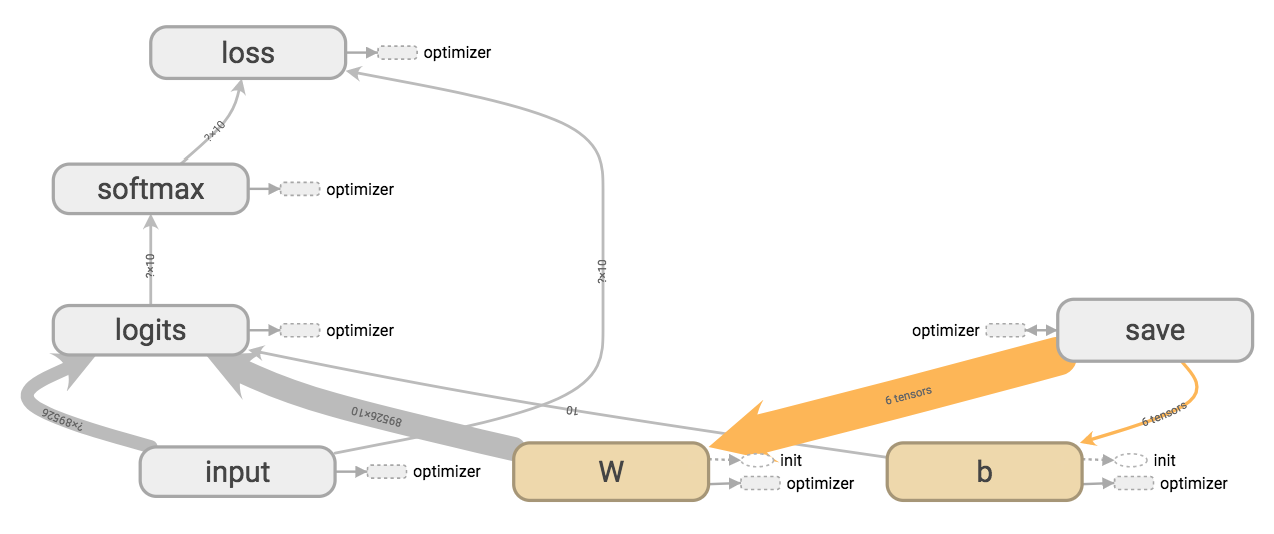
\includegraphics[width=0.45\textwidth]{figure/model_architecture}
        \caption{Our logistic regression architecture visualized with Tensorboard.}
    \end{figure}
    
    Since this model is both commonly used and simple to implement, it forms a good baseline
    for our future work. Our results for this model are reported later on in the document.

\subsubsection{Convolutional Neural Network}
\label{model:back:cnn}
    CNN uses multiple layers of convolving filters that apply on the input data and
    calculate the output after all feeding the input through all of the layers. Although
    originally built for computer vision, CNNs have shown quite significant potential in
    natural language processing (NLP), and especially in sentence classification.
    Our chosen network architecture is based upon Yoon Kim's work on sentence
    classification\cite{kim2014convolutional}. The architecture consists of four 
    main parts: a word
    embedding layer, a convolution layer, a pooling layer and a fully connected layer
    at the end.
    \begin{figure*}
    \center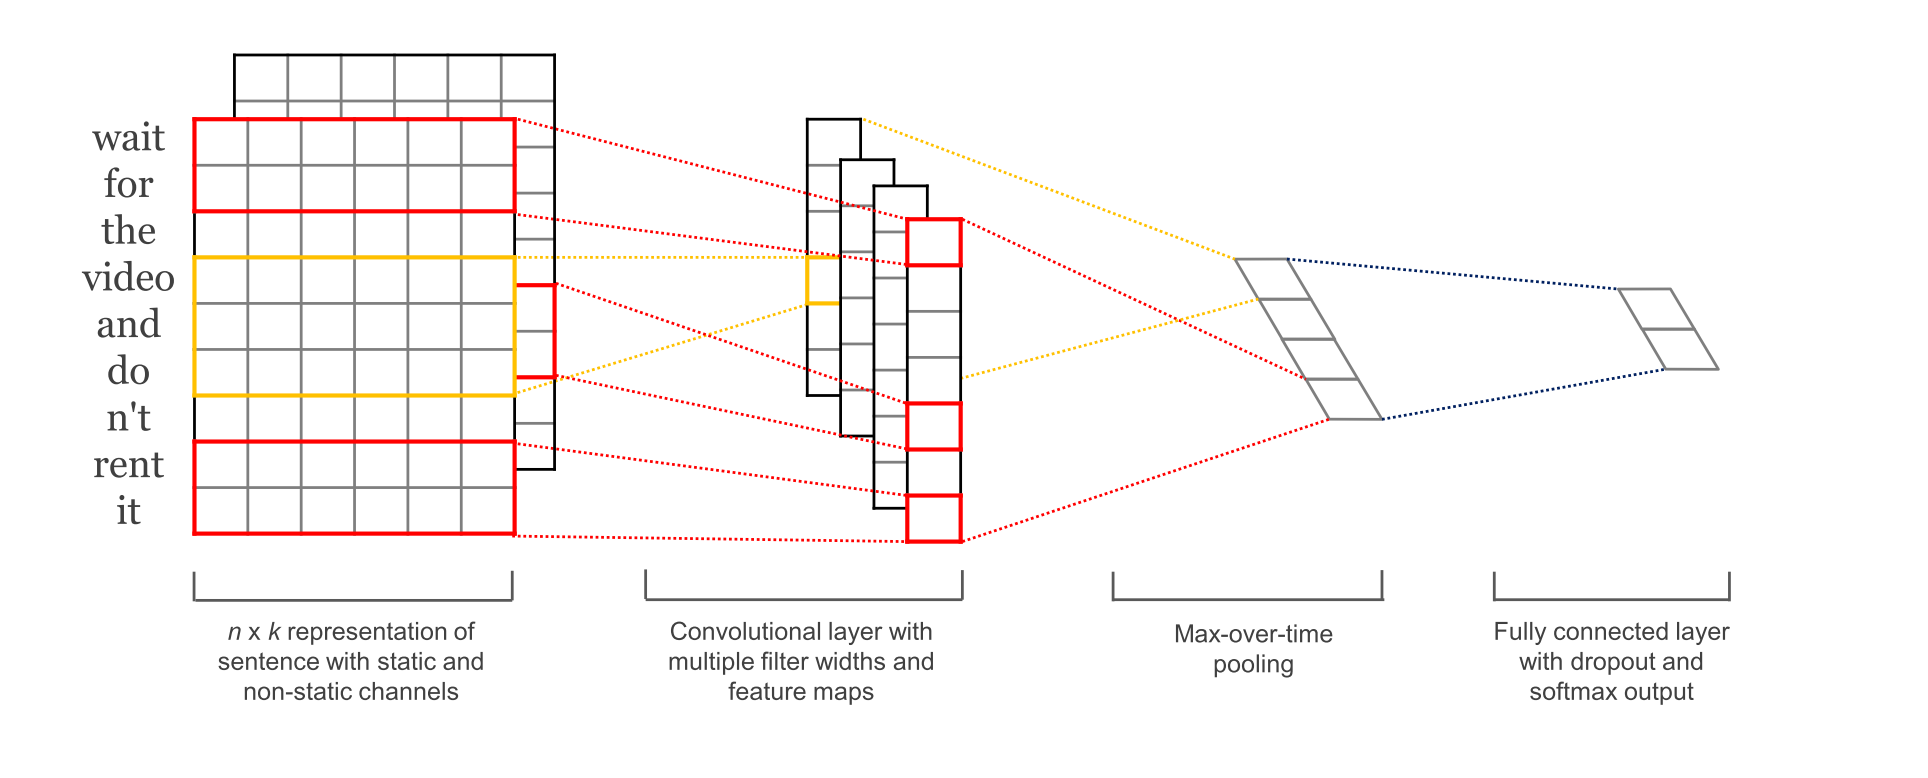
\includegraphics[width=0.9\textwidth]{figure/sc_model}
    \caption{Model architecture with two channels for an example sentence,
     figure credit: \cite{kim2014convolutional}}
    \end{figure*}

    Distributed word embeddings, proposed by Mikolov et al.
    in 2013\cite{word2vec}, allow us to represent a word as a vector in
    multi-dimensional space, and they form the basis for feeding text into our deep
    learning model.

    Let $x_{i} \in \mathbb{R}^k$ be a dimentional word vector representing the $i$-th word in the
    sentence. Thus, the sentence would be represented by
    \begin{equation}
    x_{1:n} = x_1 \oplus x_2 \oplus ... \oplus x_n
    \end{equation}
    W $\oplus$ signifies concatenation. Suppose $x_{i:i+j}$ refers to concatenating
    word vectors $x_i, x_{i+1}, ... , x_{i+j}$. The convolution operator with a filter
    $W \in \mathbb{R}^{hk}$ applied to a window size of $h$
    words is defined as
    \begin{equation}
    c_i = f(W \cdot x_{i:i_{h-1}} + b)
    \end{equation}
    W $b$ is a bias term and $f$ signifies a non linear function such as the hyperbolic
    tangent. We use this filter to generate a feature map $c = [c_1, c_2, ... ,x_{n-h+1}]$
    with $c \in \mathbb{R}^{n-h+1}$ by applying the filter to each possible window of words in
    the sentence $x_{1:h}, x_{2:h+1}, ... ,x_{n-h+1:n}$.

    We plan to use multiple filters with varying window sizes to obtain multiple features, and we will
    compare our results for different hyperparameters.
    A max-over-time pooling operation $\hat{c}$ = max\{$c$\} will be applied once the feature
    maps are generated. The pooling operation outputs the largest value from each individual
    feature maps. We will employ dropout on the penultimate layer $z = [\hat{c}_1,...,\hat{c}_m]$
    (we have $m$ filters) for regularization with a constraint on $l_2$-norms of the weight
    vectors. This should help prevent co-adaptation of hidden units by randomly setting weights
    to zero for selected neurons. The function is expressed below:

    \begin{equation}
    y = W \cdot (z \circ r) + b
    \end{equation}

    w $\circ$ is the element-wise multiplication operator and $r \in \mathbb{R}^m$ is
    the masking vector of Bernoulli random variables with probability $p$ of being 1.
    The gradients are backpropagated through the unmasked units during training. At test
    time, the learned weight vectors are scaled by $p$ such that $\hat{w} = pw$ and $\hat{w}$
    is used to score unseen sentences. Finally, we will constrain $l_2$-norms of the weight
    vectors by rescaling $w$ to have $||w||_2 = s$ whenever $||w||_2 > s$ after a gradient
    decent step.

\subsection{Stretch Goals}
\label{model:stretch}
    
    Beside the system architecture described in \autoref{model:back}, we also have a
    list of stretch goals. These include a LSTM based sentiment analysis and a 
    web-based user interface. The detail of the stretch
    goals are still yet to be fixed, and it will be will be included in the final project
    report once finished. 

\subsubsection{Long Short-Term Memory (LSTM)}
\label{model:stretch:lstm}
    The LSTM model was originally proposed by Sepp Hochreiter and J\"urgen Schmidhuber back in 
    1997\cite{hochreiter1997long}, and usually serves as a building block of larger
    recurrent neural network (RNN) layers. The basic object of LSTM is to fine-tune
    the memory length of the input and system state over an arbitrary period of time
    hence preventing premature ``memory loss'' and gradient vanishing of RNN.
    
    Given a word sequence $S=\{w_0,w_1,\ldots,w_{l-1}\}$ with length $l$, the states
    of LSTM are updated as:
    $$
    \begin{bmatrix} 
    i_t\\f_t\\o_t\\c_t 
    \end{bmatrix} = 
    \begin{bmatrix}
    \sigma\\\sigma\\\sigma\\\tanh
    \end{bmatrix}
    S[h_{t-1},x_t]
    $$
    , in which $c_t=f_t\circ c_{t-1} + i_t\circ\hat{c_t}$ and $h_t=o_t\circ\tanh{c_t}$.
    At time $t$ in this relationship, $c_t$ and $h_t$ are the LSTM memory and 
    hidden state, $\hat{c_t}$ is the current cell state. The input at time $t$ 
    is $x_t$ and the input/forget/output gate activation are represented by $i$, 
    $f$ and $o$ respectively. $\sigma$ and $\circ$ are notations of logistic 
    sigmoid function and element-wise multiplication\cite{zhou2016text}.
    
    Depending on the requirement on system causality, the LSTM can be applied on
    both directions of time, which becomes Bidirectional LSTM 
    (BLSTM)\cite{schuster1997bidirectional,barnes2017assessing}.

\subsubsection{Web Interface}
\label{model:stretch:web}
    To improve the user-friendliness of this project, we also plan to create a 
    web-based user interface for the program. With a webpage, selecting
    the model for sentiment analysis can be done in a mouse click instead of 
    enter a series of command line parameters, the output can also
    be read from web browser, not a standard output stream in terminal. 

\section{Performance Evaluation}
\label{performance}
    \begin{table*}[]
        \centering
        \caption{Initial Results from BoW Models}
        \label{my-label}
        \begin{tabularx}{\textwidth}{ X  X  X X  X }
        \toprule
        Method & Binomial Training & Binomial Testing & Multinomial Training & Multinomial Testing \\
        \midrule
        scikit-learn LR & 0.9981 & \textbf{0.8697} & N/A & N/A \\
        tensorflow LR & 0.8670 & 0.8583 & 0.9982 & \textbf{0.3734} \\
        \bottomrule
        \end{tabularx}
    \end{table*}
\subsection{Experiment Setup}
    In order to evaluate our baseline sentiment analysis model, we used the
    Stanford Large Movie Review data set \cite{maas2011learning}. This data
    set consists of 50,000 movie reviews and corresponding scores from IMDb.
    25,000 reviews are designated for training, and 25,000 reviews are designated for testing.
    T are a total of 89526 unique words used in the interviews, and each
    movie rating is an integer between 1 and 10. Using this dataset, we preform
    two different machine learning tasks. First, we predict whether a movie review
    has a mostly positive or mostly negative attitude towards the movie of interest. 
    Second, we predict the score of unlabeled movie reviews from 1-10. We treat
    both cases as instances of the multiclass classification problem.
    
    The whole project was coded with python 3, and our evaluation was conducted on
    a Ubuntu 14.04 LTS machine with a 3.1GHz Intel Core i7 CPU with 8MB cache,
    6GB RAM, and a 4GB nVidia GTX 1050 GPU.
    
\subsection{Performance Metrics}
    To measure the performance of our systems, we calculate the raw accuracy
    scores of the systems. We divide the number of correct class predictions
    by the total number of predictions made. Accuracies were calculated
    for both the training and testing sets of the Stanford Large Movie Review dataset.
    
\subsection{Experiment Results}
    In Table 1 we provide initial results for our baseline bag of words model using
    two different machine learning toolkits. The first set of results come from
    using the python scikit-learn package's built in logistic regression model.
    This model relies on highly optimized logistic regression algorithms
    contained in the liblinear \cite{Fan:2008:LLL:1390681.1442794} package,
    and it quickly converged to the global minimum. Since logistic regression
    can be treated as convex optimization problem, we do not have to worry 
    about escaping local optima. We also evaluated the logistic regression
    model using a custom tensorflow implementation. The results reported
    above were achieved training our model with a 20 shuffled epochs, a
    batch size of 50, a learning rate of \num{1e-4}, and the Adam optimizer.
    In the binomial case, our model is given training data w samples are
    labeled only as positive (the rating is $\leq 5$) or negative (the rating is
    $\geq 6$), and the ground truth score is hidden. We found that this slightly
    increased our accuracy compared to predicting scores from 1-10 and
    bucketing the scores afterwards. In the multinomial case, our model is
    shown the complete rating and predicts scores from 1-10.
    
    While the scikit-learn package included a highly optimized algorithm for
    preforming binomial linear regression, none of the included solvers were
    capable of handling the multinomial linear regression problem due to intensive
    memory usage. Thus we have only provided results from our tensorflow
    model in the multinomial case.
\subsection{Future Experiments}
    In addition to using the above data set, we will also train and test using the 
    Stanford Sentiment Treebank, which is one of the data sets Kim evaluated in 
    his paper\cite{sentimenttreebank}. Using the same data set
    will allow us to compare our model with Kim's model directly. 
    Both binary (positive/negative) and fine-grained (scale from 1-5) 
    classification tasks will be performed and scored for accuracy.
    For all tasks, we will compute the accuracy of our model by diving the 
    number of correct classifications by the total number of test samples.
    
    Since we are already able to get good binomial classification results with a simple
    model and a large dataset, it will be interesting to see how much a neural network
    will be able to improve upon the baseline. In addition, it will be interesting to
    to examine how will the models generalize across datasets. From the results
    above we can see that the Logistic Regression model overfits on the multinomial
    regression model, so a more fair comparison might include a model that has
    an additional regularization term added to its cost function.
    
\section{Simulation Environment and Result}
\label{simulation}

\section{Web-based Real-time Sentiment Analysis}
\label{web}

\section{Conclusion}
\label{conclusion}

%
%
%
%\section{Current Progress and Project Management}
%\label{manage}
%
%\subsection{Current Status \& Team Coordination}
%\label{manage:status}
%    The course project has been overall well maintained and tracked. 
%    The whole project including documents and source code are stored
%    in a git repository hosted on GitHub 
%    (\url{https://github.com/ufjfeng/EEL6935-Course-Project}),
%    hence the contribution of each team member had been tracked.
%    
%    The current project status is:
%    \begin{description}
%        \item[\CheckedBox] Choose topic
%        \item[\CheckedBox] Write proposal
%        \item[\CheckedBox] Gather dataset
%        \item[\CheckedBox] Build baseline model with Logistic Regression
%        \item[\CheckedBox] Write mid-term report 
%        \item[$\Box$] Build CNN model
%        \item[$\Box$] (stretch) Build LSTM model
%        \item[$\Box$] (stretch) Build web interface
%        \item[$\Box$] Write project documentation
%        \item[$\Box$] Write final report
%    \end{description}
%
%\subsection{Weekly Plans and Deliverables}
%\label{manage:plan}
%
%    \begin{center}
%        \begin{tabular}{| l | p{7cm} |}
%        \hline
%        Week & Plan \\ \hline
%        1-3 & Read paper and select project topic \\ \hline
%        4 & Write project proposal and make slides \\ \hline
%        6-8 & Build project baseline model and finalize design \\ \hline
%        9 & Write midterm project report and make slides \\ \hline
%        10-13 & Build CNN model and work on stretch goals \\ \hline
%        14-15 & Finalize course project, collect data and write final report \\ \hline
%        \end{tabular}
%    \end{center}
%
%    By the end of this semester, we will dilever:
%    \begin{itemize}
%    \item A working program for sentiment analysis and related documents
%    \item Final report of the project
%    \item Slides for in-class presentation
%    \item GitHub repository
%    \end{itemize}

\bibliographystyle{IEEEtran}
\bibliography{eel6935_final.bib}

\end{document}
